\documentclass{article}

%
% 引入模板的style文件
%
\usepackage{homework}

\setCJKmainfont{SimSun}[AutoFakeBold] %宋体加粗
\setCJKsansfont{SimHei}[AutoFakeBold] %黑体加粗


\usepackage{minted} %配合minted宏包进行好看的高亮
\usepackage{currfile} %配合minted宏包进行好看的高亮
\usepackage{caption} %配合minted宏包进行好看的高亮
\usepackage{tcolorbox} %配合minted宏包进行好看的高亮
\usepackage{xcolor} %配合minted宏包进行好看的高亮
\tcbuselibrary{skins} %配合minted宏包进行好看的高亮
\tcbuselibrary{minted} %配合minted宏包进行好看的高亮
\usemintedstyle{paraiso-dark} %配合minted宏包进行好看的高亮
\usepackage{framed} 


%
% 封面
%


\title{
	
\includegraphics[width=0.5\textwidth]{images/title/ucas_logo 1.pdf}\\
    \vspace{1in}
    \textmd{\textbf{\hmwkClass}}\\
	\textmd{\Large{\textbf{\hmwkClassID}}}\\
    \textmd{\textbf{\hmwkTitle}}\\
    \normalsize\vspace{0.1in}\large{\hmwkCompleteTime }\\
    \vspace{0.1in}\large{\textit{\hmwkClassInstructor\ }}\\
    \vspace{1in}
	
\includegraphics[width=0.25\textwidth]{images/title/Cyber.jpg}\\
	\vspace{1in}
}

\author{
	\hmwkAuthorName \\ 
	\hmwkAuthorStuID \\
	\hmwkAuthorInst \\
	\hmwkAuthorzhuanye \\
	\hmwkAuthorfangxiang
	}
\date{}

\renewcommand{\part}[1]{\textbf{\large Part \Alph{partCounter}}\stepcounter{partCounter}\\}


%
% 正文部分
%
\begin{document}


\maketitle


%\include{chapters/ch01}
%\include{chapters/ch02}
%\include{chapters/ch03}
%\include{chapters/ch04}
%\include{chapters/ch05}


\begin{homeworkProblem}
	两个各有$n$个数值元素的独立数据库, 假设你(持有数值$k$)可以用$O(1)$的时间在其中任意一个数据库(一次)查询出第$k$小的元素\footnote{可以将这两个数据库都视作\textbf{预言机(Oracle Machine)}, 即为可以在单一运算之内解答特定问题的黑盒式数据库.}. 现要求以$O(\log n)$($n$为查询次数)的时间来确定这两个数据库(共$2n$个元素)的中位数(即第$n$小的元素).
	\\
	
	\solution 算法的思路是在第1个数据库中找出1个元素$a_i$, 在第2个数据库中找出1个元素$b_j$, 并保证小于等于$a_i$和$b_j$的元素总数为$N$个, 然后在所有小于$a_i$的元素中找出最大的元素$a_m$, 在所有小于$b_j$的元素中找出最大的元素$b_n$, 两个数据库所有的元素中第$n$小的元素就是$\text{max}(a_m,b_n)$. 算法\ref{alg:FindMedian}的伪代码描述如下:
	\begin{algorithm}[H]
		\begin{algorithmic}[1]
		\Require{数据库$A$和数据库$B$及预言机\textbf{Oracle}}
		\Ensure{两个数组中的中位数(即第$n$小的元素)}
		\State \textbf{int} $i=1$, $j=n$;
		\If{$a[n]\leq b[1]$} \Comment{使用\textbf{Oracle}查询数据库$A$中第$n$小的元素$a[n]$和$B$中第1小的元素$b[1]$}
			\State \Return $a[n]$;
		\EndIf
		\If{$a[1]\geq b[n]$} \Comment{使用\textbf{Oracle}查询数据库$A$中第$1$小的元素$a[1]$和$B$中第$n$小的元素$b[n]$}
			\State \Return $b[n]$;
		\EndIf
		\While{$j\geq 3$}
			\State \textbf{int} $k:=(i+j)/2$;
			\State \textbf{int} flag = $a[k]-b[n-k+1]$; \Comment{使用\textbf{Oracle}查询$a[k]$和$b[n-k+1]$}
			\If{flag $>0$}
				\State $j:=k$;
			\ElsIf{flag $<0$}
				\State $i:=k$;
			\Else
				\State \Return $a[k]$;
			\EndIf
		\EndWhile
		\State \Return $\text{max}(a[k], b[n-k])$;
		\State \textbf{end \{FindMedian\}}
		\end{algorithmic}
		\caption{算法$\textbf{FindMedian}(A, B)$}
		\label{alg:FindMedian}
	\end{algorithm}
	设数据库$A$中第$k$小的元素为$a_k$, 数据库$B$中第$k$小的元素为$b_k$, 定义函数$f$: $f(k) = a_{k} - b_{n - k + 1}$, 显然$f(k)$是关于$k$的单调递增函数. 特别地, 当$f(1) \geq 0$时, $b_n$就是第n小的元素; 当$f(n) \leq 0$时, $a_n$就是第n小的元素. 若能找到一个$k$, 使得: ${f(k) \leq 0}$且$f(k + 1) \geq 0$. 这表明: $a_1 \leq ... \leq a_k \leq b_{n - k + 1}$且$b_1 \leq ... \leq b_{n-k} \leq a_{k+1}$. 设集合$S=\{a_1,a_2,...,a_k,b_1,b_2,...,b_{n-k}\}$, $S$的元素个数为$n$. 由上可知: $\text{max}(a_k,b_{n-k})$就是第$n$小的元素. 显然查询次数的函数$K$满足递推方程: $K(n) = K(n/2) + O(1)$, 根据主定理解得$K(n)=O(\log n)$(其中$n$为查询次数). 
	
	\textbf{注释:} 如果不使用预言机, 而是调用\textbf{PartSelect}算法, 则查询第$k$小元素的需要消耗$O(n)$的时间(课上讲过), 从而\textbf{FindMedian}算法的时间复杂度递推方程为$T(n)=T(n/2)+O(n)$, 解得$T(n)=O(n)$(其中$n$为数据库元素个数).
	\newpage
\end{homeworkProblem}


\pagebreak

\begin{homeworkProblem}
	给定一个二叉树$T$, 请给出一个$O(n)$算法来反转二叉树. 例如下面图\ref{fig:翻转二叉树}反转左二叉树, 我们得到右二叉树.
	\begin{figure}[H]  % 这里记得用[H]
		\centering
		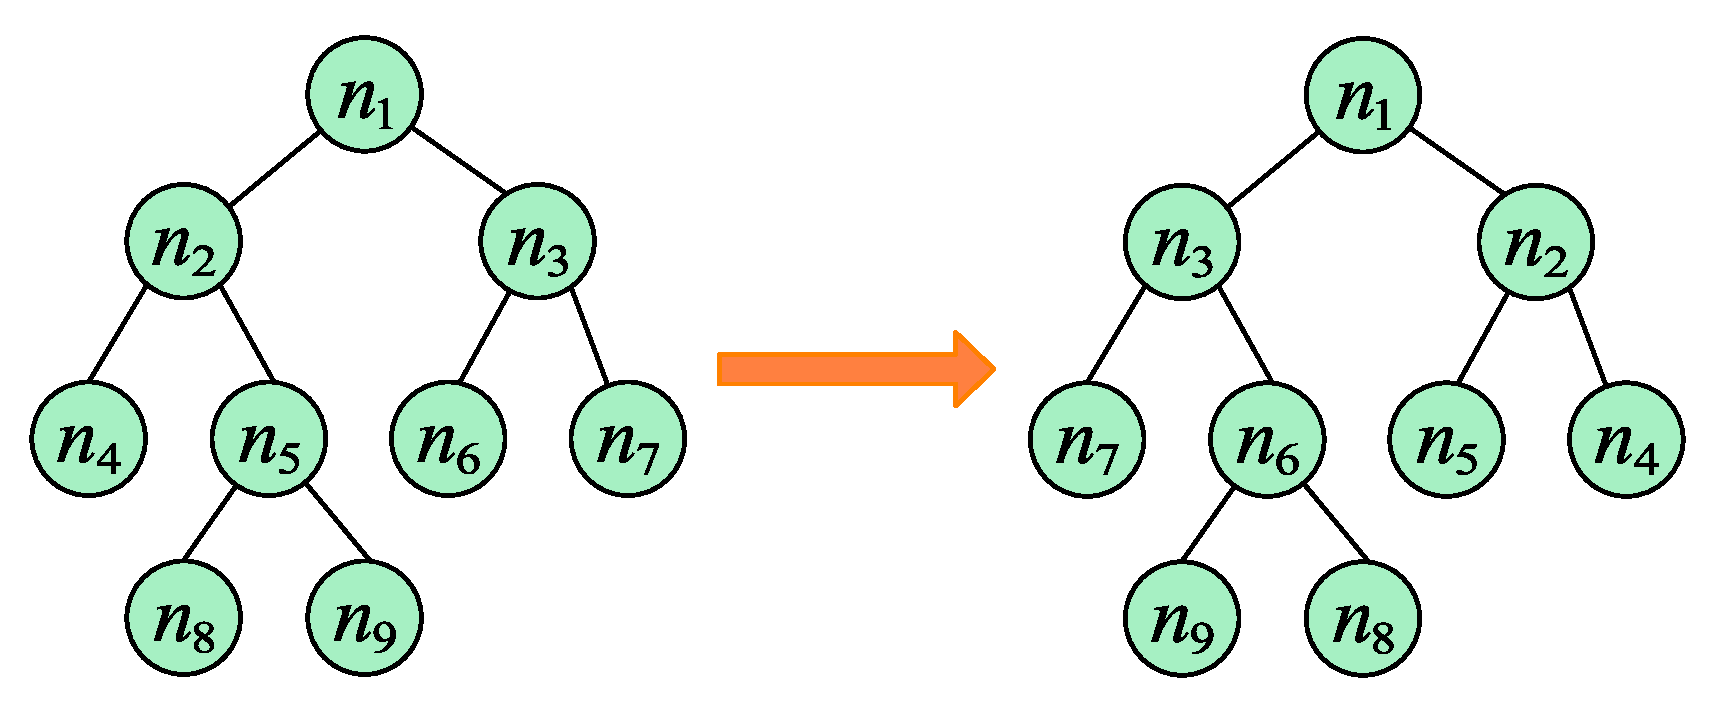
\includegraphics[width=0.5\textwidth]{images/title/翻转二叉树.pdf}
		\caption{翻转二叉树}
		\label{fig:翻转二叉树}
	\end{figure}

	\solution 这是一道很经典的二叉树问题. 显然, 我们从根节点开始, 递归地对树进行遍历, 并从叶子节点先开始翻转. 如果当前遍历到的节点root的左右两棵子树都已经翻转, 那么我们只需要交换两棵子树的位置, 即可完成以root为根节点的整棵子树的翻转. 算法对应的伪代码过于简单就不予描述了, 直接给出其C++代码:
\begin{tcblisting}{listing engine=minted,boxrule=0.1mm,
colback=blue!5!white,colframe=blue!75!black,
listing only,left=5mm,enhanced,sharp corners=all,
overlay={\begin{tcbclipinterior}\fill[red!20!blue!20!white] (frame.south west)
rectangle ([xshift=5mm]frame.north west);\end{tcbclipinterior}},
minted language=c++,
minted style=tango,
minted options={fontsize=\small,breaklines,autogobble,linenos,numbersep=3mm}}
struct TreeNode {
    int val;
    TreeNode *left;
    TreeNode *right;
    TreeNode() : val(0), left(nullptr), right(nullptr) {}
    TreeNode(int x) : val(x), left(nullptr), right(nullptr) {}
    TreeNode(int x, TreeNode *left, TreeNode *right) : val(x), left(left), right(right) {}
};
/*以上是二叉树的ADT定义*/
TreeNode* invertTree(TreeNode* root) {
    if (root == nullptr) {
        return nullptr;
    }
    TreeNode* left = invertTree(root->left);
    TreeNode* right = invertTree(root->right);
    root->left = right;
    root->right = left;
    return root;
}
\end{tcblisting}
	现在分析一下时空复杂度: 由于要遍历二叉树中的每个节点, 且在其上交换两颗子树的时间是常数, 所以时间复杂度为$T(n)=O(n)$; 递归所使用的栈空间主要由递归栈的深度决定, 而递归栈的深度就等于二叉树的高度(即$\log n$), 但最坏情形下树形呈链状, 则递归栈深度为$O(n)$, 所以空间复杂度为$O(n)$.
\end{homeworkProblem}

\pagebreak

\begin{homeworkProblem}
	监狱有$N$个房间, 每个房间关押一个犯人, 有$M$种宗教, 每个犯人会信仰其中一种. 如果相邻房间的犯人的宗教信仰相同, 就可能发生越狱, 求有多少种状态可能发生越狱. 例如, 有3个房间和2种宗教,然后会发生6种不同的状态. 
	\\

	\solution 这本质上就是个排列组合问题. 每个房间的犯人都有$M$中信仰, 故总的状态数为$M^N$. 根据题意, 只要有一对相邻房间的犯人宗教信仰相同, 则就会发生越狱事件. 
	考虑越狱的状态数会比较复杂, 所以\textbf{正难则反}(容斥原理), 考虑不发生越狱\footnote{即任意相邻房间对的犯人宗教信仰都不相同.}的状态数: 第1个房间的犯人有$M$种选择, 而第2个房间的犯人有$M-1$种选择, 且第3个房间的犯人有$M-1$种选择\footnote{只要第3个房间犯人的信仰跟第2个房间犯人的信仰不同即可, 即使跟第1个房间相同也没事(因为不相邻而不会发生越狱).}, 同理第4个房间的犯人也有$M-1$种选择$\cdots$. 因此, 不发生越狱的状态数为$M\cdot (M-1)^{N-1}$, 从而越狱的状态数为$M^N-M\cdot (M-1)^{N-1}$. 

	显然$O(1)$的公式已经给出来了, 接下来只需要套一下快速幂的模板(递归+分治)即可:
	\begin{algorithm}[H]
		\begin{algorithmic}[1]
		\Require{正实数$x$ (double), 正整数$N$ (long long)}
		\Ensure{$x^N$}
		\If{$N$ == 0} \Comment{递归终止条件为$N=0$}
			\State \Return 1.0;
		\EndIf
		\State \textbf{double} $y=\textbf{QuickMul}(x, N/2)$; \Comment{要计算$x^N$时,先递归地计算出$y = x^{\lfloor N/2 \rfloor}$}
		\If{$N\%2 $ == 0} \Comment{如果$N$为偶数, 则$x^N=y^2$}
			\State \Return $y\ast y$; 
		\Else \Comment{如果$N$为奇数, 则$x^N=y^2\times x$}
			\State \Return $y \ast y \ast x$; 
		\EndIf
		\State \textbf{end \{QuickMul\}}
		\end{algorithmic}
		\caption{算法$\textbf{QuickMul}(x, N)$}
		\label{alg:QuickMul}
	\end{algorithm}
	最后只需要调用一下即可: \textbf{return} $\textbf{QuickMul}(M, N)-M\ast \textbf{QuickMul}(M-1, N-1)$. 上述伪代码稍微改一下就可以写出C++代码, 就不予以展示了. 显然, 此公式调用了两次快速幂算法\footnote{快速幂算法需要$O(\log N)$的时间和$O(\log N)$的空间.}, 所以该问题解法的时间复杂度为$T(N)=O(\log N)+O(\log N)=O(\log N)$, 空间复杂度$S(N)=O(\log N)$.
	\newpage
\end{homeworkProblem}

\pagebreak

\begin{homeworkProblem}
	给定一棵二叉树, 假设两个相邻节点之间的距离为1, 请给出求解二叉树中任意两个节点的最大距离的方法.

	\solution \textbf{此题即求二叉树的直径}, 任意一条路径均可以被看作由某个节点为起点, 从其左儿子和右儿子向下遍历的路径拼接得到. 如下图\ref{fig:路径的看法示意图}, 我们可以知道路径$[9,4,2,5,7,8]$可以被看作以$2$为起点, 从其左儿子向下遍历的路径$[2,4,9]$和从其右儿子向下遍历的路径$[2,5,7,8]$拼接得到.
	\begin{figure}[H]  % 这里记得用[H]
		\centering
		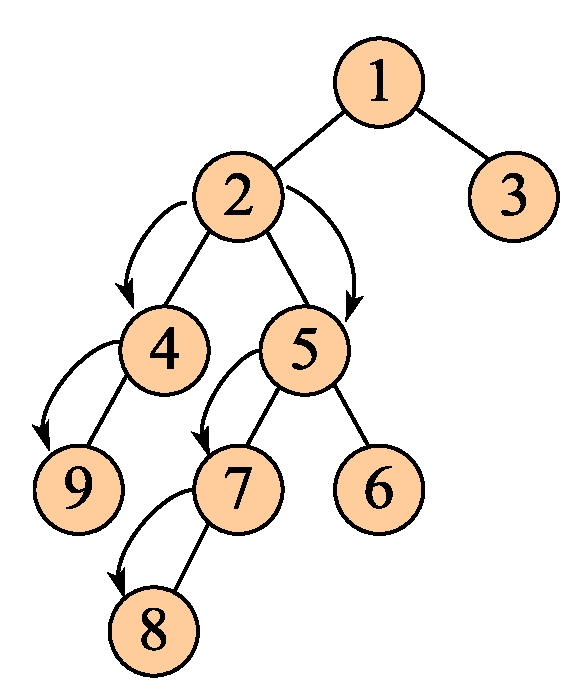
\includegraphics[width=0.25\textwidth]{images/title/二叉树直径.pdf}
		\caption{路径的看法示意图}
		\label{fig:路径的看法示意图}
	\end{figure}
	
	我们利用\textbf{深度优先搜索(dfs)}来遍历这颗二叉树, 对于所遍历到的每个非叶子节点: 再计算求得以其左儿子为根的子树深度$L$和右儿子为根的子树深度$R$, 则以该节点为起点的路径长度的最大值(即以该节点为根的子树的直径)为$L+R$. 
	
	而计算以node节点为根的子树深度: 我们可以定义递归函数$\textbf{dfs}(\text{node})$, 先递归调用该函数求得以node左儿子和右儿子为根的子树深度$L,R$, 则返回以node节点为根的子树深度$\text{max}(L,R)+1$.

	最后递归搜索(dfs)这颗二叉树的每个节点, 并设置全局变量Diam来记录并更新迭代各节点对应的子树直径, 从而求得整个二叉树的最大直径. 算法伪码(C++代码与此类似, 就不罗列了)描述如下:

	\begin{algorithm}[H]
		\begin{algorithmic}[1]
		\Require{一棵二叉树root} \Comment{TreeNode数据类型的定义在前面已给出}
		\Ensure{二叉树root的直径Diam}
		\State \textbf{global} Diam = 0; \Comment{定义全局变量来记录并更新以各节点为根的子树直径的最大值}
		\If{node == \textbf{null}} \Comment{递归终止条件}
			\State \Return 0; \Comment{以叶子节点为根的子树深度为0}
		\EndIf
		\State \textbf{int} Left = \textbf{dfs}(node$\rightarrow$left); \Comment{递归计算以node左儿子为根的子树深度}
		\State \textbf{int} Right = \textbf{dfs}(node$\rightarrow$right); \Comment{递归计算以node右儿子为根的子树深度}
		\State $\text{Diam} = \textbf{max}(\text{Left}+\text{Right}, \text{Diam})$; \Comment{更新迭代子树直径以求得最大值(即整个二叉树的直径)}
		\State \Return $\textbf{max}(\text{Left},\text{Right})+1$; \Comment{返回以当前节点为根的子树深度}
		\State \textbf{end \{dfs\}}
		\end{algorithmic}
		\caption{算法$\textbf{dfs}(\text{TreeNode}\,\,\text{node})$}
		\label{alg:dfs}
	\end{algorithm}
	现在来分析以下算法的复杂度: 深度优先搜索二叉树, 时间复杂度显然就是$O(N)$($N$为二叉树的节点个数); 由于递归函数在递归过程中需要为每一层递归函数分配栈空间, 所以这里需要额外的空间且该空间取决于递归的深度, 而递归的深度显然为二叉树的高度, 并且每次递归调用的函数里又只用了常数个变量, 所以所需空间复杂度为$O(H)$($H$为二叉树的高度). 
\end{homeworkProblem}

\pagebreak

\begin{homeworkProblem}
	请给出三路快速排序的算法 (算法的时间复杂度显然仍是$O(n\log n)$, 空间复杂度为$O(\log n)$).

	\solution 一趟三路快排的结果: 随机化选取一个pivot, 完成一趟三路快排, 数组会分为低($<$pivot的元素)、中($=$pivot的元素)、高($>$pivot的元素)三个分区. 一趟三路快排的思想核心是\textbf{三指针}, 具体来说是先将随机化选取好的pivot放到数组头部, pivot紧右边的是低分区, 然后是中分区, 再然后是未知区域, 数组最右边的是高分区. 指针$lt$用来控制低分区的扩张, 指针$gt$用来控制高分区的扩张, 指针$i$用来遍历未知区域(具体如下图\ref{fig:三路快排分区示意图}(a)中所示). 一趟三路快排需用\textbf{while}循环, 循环条件为$i<gt$. 当指针$i$所指元素$\text{nums}[i]$==pivot时, 中分区扩张(即$i$++); 当$\text{nums}[i]>$pivot时, 交换$\text{nums}[i]$和$\text{nums}[gt-1]$以使得元素$\text{nums}[i]$向高分区靠拢, 然后高分区扩张(即$gt$-\,-), 此时指针$i$不用动, 因为换过来的还是未知元素(需要继续检索); 当$\text{nums}[i]<$pivot时, 交换$\text{nums}[i]$和$\text{nums}[lt+1]$以使得元素$\text{nums}[i]$向低分区靠拢, 与此同时低分区扩张(即$lt$++), 且此时指针$i$所指元素是已知的($=$pivot), 所以需要$i$++来继续检索未知区域. 经过一趟三路快排则数组演变为下图\ref{fig:三路快排分区示意图}(b)中所示. 算法伪代码见如下\footnote{当数组中存在大量的重复元素时, 双路快排的交换操作就显得很多余, 而三路快速排序恰好能解决这个问题.}:
	\begin{figure}[H]  % 这里记得用[H]
		\centering
		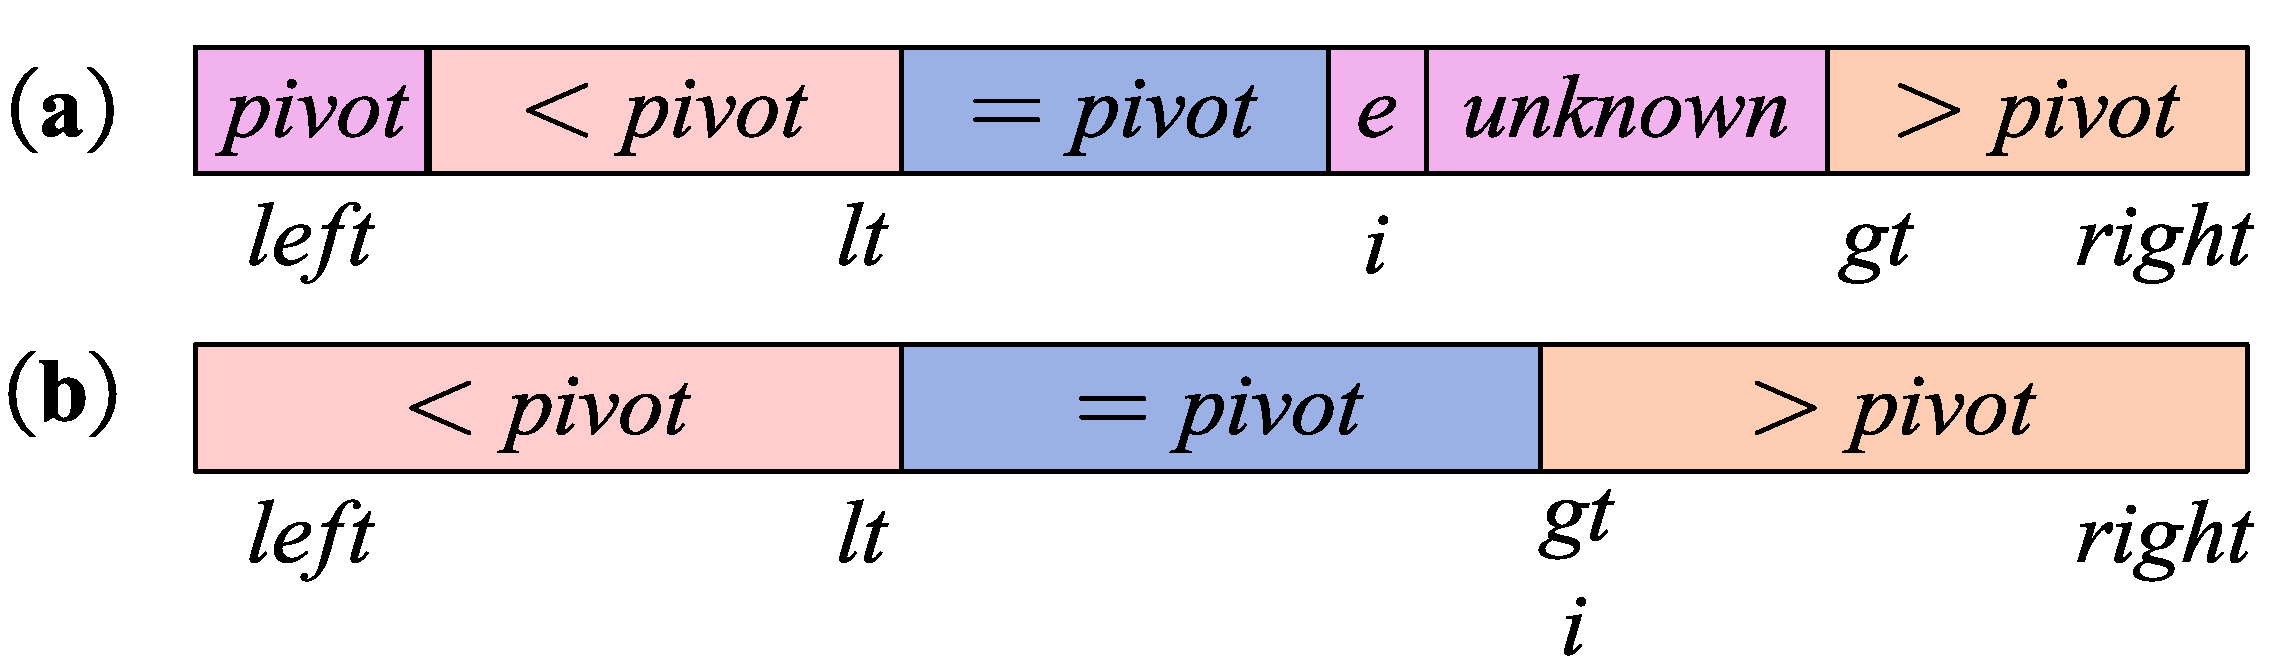
\includegraphics[width=0.6\textwidth]{images/title/三路快速排序.pdf}
		\caption{三路快排分区示意图}
		\label{fig:三路快排分区示意图}
	\end{figure}
	\begin{algorithm}[H]
		\begin{algorithmic}[1]
		\Require{数组$A[0,\cdots,n - 1]$的子段$A[\text{left}, \text{right}]$}
		\Ensure{排序后的数组子段$A[\text{left}, \text{right}]$}
		\If{left >= right} \Comment{递归终止条件}
			\State \Return;
		\EndIf
		\State \textbf{int} rand_index = left + rand()$\%$(right $-$ left + 1); \Comment{随机化选取主元pivot}
		\State \textbf{swap}($A$[left], $A$[rand_index]); \Comment{将选好的主元放到数组左端}
		\State \textbf{int} pivot = $A$[left];
		\State \textbf{int} lt = left $-$ 1, $i$ = left, gt = right + 1; \Comment{三指针的初始化}
		\While{$i<\text{gt}$} \Comment{当指针$i$和指针$gt$对撞时结束循环}
			\If{$A[i]$ == pivot}
				\State $i$++; \Comment{此时只需扩张中分区}
			\ElsIf{$A[i]$ > pivot} \Comment{此时使元素$\text{nums}[i]$向高分区靠拢并扩张高分区}
				\State \textbf{swap}($A[i],A[\text{gt}-1]$), gt$\text{-\,-}$; \Comment{并且指针$i$不动来继续检索当前所指的未知元素}
			\ElsIf{$A[i]$ < pivot} \Comment{此时令元素$\text{nums}[i]$向低分区靠拢并扩张低分区}
				\State \textbf{swap}($A[\text{lt}+1],A[i]$), lt$\text{++}$, $i\text{++}$; \Comment{并且指针$i$继续向前(右移一位)检索未知元素}
			\EndIf
		\EndWhile
		\State \textbf{QuickSort3}($A$, left, lt); \Comment{继续递归地对左边数组进行快排}
		\State \textbf{QuickSort3}($A$, gt, right); \Comment{继续递归地对右边数组进行快排}
		\State \textbf{end \{QuickSort3\}}
		\end{algorithmic}
		\caption{三路快速排序\textbf{QuickSort3}算法}
		\label{alg:三路快速排序}
	\end{algorithm}
	\newpage
	以下是三路快排的C++代码, 使用的话只需要执行\textbf{QuickSort3}(nums, 0, nums.size() $-$ 1)即可.
\begin{tcblisting}{listing engine=minted,boxrule=0.1mm,
colback=blue!5!white,colframe=blue!75!black,
listing only,left=5mm,enhanced,sharp corners=all,
overlay={\begin{tcbclipinterior}\fill[red!20!blue!20!white] (frame.south west)
rectangle ([xshift=5mm]frame.north west);\end{tcbclipinterior}},
minted language=c++,
minted style=tango,
minted options={fontsize=\small,breaklines,autogobble,linenos,numbersep=3mm}}
#include<iostream>
#include<algorithm>
#include<vector>
using namespace std;
void QuickSort3(vector<int>& nums, int left, int right) {
    if(left >= right) {
        return;
    }
    int rand_index = left + rand()%(right - left + 1);
    swap(nums[left], nums[rand_index]);
    int pivot = nums[left];
    int lt = left - 1, i = left, gt = right + 1;
    while(i < gt) {
        if(nums[i] == pivot) {
            i++;
        }
        else if(nums[i] > pivot) {
            swap(nums[i], nums[gt - 1]);
            gt--;
        }
        else if(nums[i] < pivot) {
            swap(nums[lt + 1], nums[i]);
            lt++, i++;
        }
    }
    QuickSort3(nums, left, lt);
    QuickSort3(nums, gt, right);
}
\end{tcblisting}
并且借助一趟三路快排的思想可以解决\textbf{荷兰三色国旗问题}(伪码见如下算法\ref{alg:三色国旗算法})且能优化"选取第$k$小元素"的算法.
\begin{algorithm}[H]
	\begin{algorithmic}[1]
	\Require{$n$个实数构成的数组$A[0,\cdots,n - 1]$}
	\Ensure{负数排在正数前面且0排在中间的数组$A[0,\cdots,n - 1]$}
	\State \textbf{int} pivot = 0;
	\State \textbf{int} lt = $-1$, $i$ = 0, gt = $n$;
	\While{$i<\text{gt}$}
		\If{$A[i]$ == pivot}
			\State $i$++;
		\ElsIf{$A[i]$ > pivot}
			\State \textbf{swap}($A[i],A[\text{gt}-1]$), gt$\text{-\,-}$;
		\ElsIf{$A[i]$ < pivot}
			\State \textbf{swap}($A[\text{lt}+1],A[i]$), lt$\text{++}$, $i\text{++}$;
		\EndIf
	\EndWhile
	\State \textbf{end \{ThreeColor\}}
	\end{algorithmic}
	\caption{三色国旗问题的\textbf{ThreeColor}算法}
	\label{alg:三色国旗算法}
\end{algorithm}
\end{homeworkProblem}

\pagebreak

\begin{homeworkProblem}
	有$n$条绳子, 它们的长度分别为$L_i$. 如果从它们中切割出$m$条长度相同的绳子, 这$m$条绳子每条最长能有多长?
	\\

	\solution 一个很直接的想法: 假如所切长度选的较短, 那么切割出来的段数就会$\geq m$; 假如所切长度选的较长, 那么切割出来的段数就会$<m$. 所以我们需要通过在区间$[0,\textbf{INT_MAX}]$中对所切长度进行二分搜索. \textbf{搜索(二分)准则}是: 取所切长度为区间中值(mid), 按照此长度计算所有绳子中切出来的段数总和, 如果段数总和$\geq m$, 则解位于右半区间(即所切长度选短了)\footnote{也可以认为此情形下的mid值就是\textbf{可行解}, 但不是\textbf{最优可行解}. 也就是说, 我们需要在另一半区间中继续二分搜索来找出\textbf{最优可行解}.}; 若段数总和$<m$, 则解位于左半区间(即所切长度选长了). 于是我们可以给出以下算法\ref{alg:切绳子}的伪代码: 
	\begin{algorithm}[H]
		\begin{algorithmic}[1]
		\Require{$n$个绳子长度构成的数组$L[0,\cdots,n - 1]$}
		\Ensure{割出$m$条最大长度且长度相同的绳段}
		\State \textbf{int} low = 0, high = \textbf{INT_MAX}; \Comment{初始化搜索区间}
		\While{low $\leq$ high}
			\State \textbf{int} mid = (low + high) $>>$ 1;
			\If{mid == 0} 
				\State \textbf{break}; \Comment{这是因为后面计算段数总和时, 分母是不能为零的!}
			\EndIf
			\State \textbf{int} cnt = 0; \Comment{每次循环都需清0}
			\For{\textbf{int} $i=0$; $i<n$; $i$++}
				\State cnt += $\left\lfloor L[i]/\text{mid}\right\rfloor $; \Comment{计算所有绳子按当前mid值所切的段数总和}
			\EndFor
			\If{cnt $\geq m$} \Comment{舍弃左半区间, 在右半区间搜索最优可行解}
				\State low = mid + 1;
			\Else \Comment{舍弃右半区间, 在左半区间搜索最优可行解}
				\State high = mid $-$ 1;
			\EndIf
		\EndWhile
		\State \Return high; \Comment{返回所找到的最优可行解}
		\State \textbf{end \{CutRope\}}
		\end{algorithmic}
		\caption{切绳子\textbf{CutRope}算法}
		\label{alg:切绳子}
	\end{algorithm}
	不妨设$n$条绳子中的长度最大值为$L_{\text{max}}$, 则搜索区间可初始化为$[0,L_{\text{max}}]$, 于是\textbf{CutRope}算法(二分)的时间复杂度显然为$O(\log L_{\text{max}})$, 算法只需要常数级的额外辅助空间, 故空间复杂度为$O(1)$.

	至此, Chap 2的作业解答完毕.
	\begin{figure}[H]  % 这里记得用[H]
		\centering
		
\includegraphics[width=0.7\linewidth]{images/title/ucas_logo 1.pdf}
		%\caption{ucas-logo}
		\label{fig:ucas-logo}
	\end{figure}
\end{homeworkProblem}



% 引用文献
\bibliographystyle{unsrt}  % unsrt:根据引用顺序编号
\bibliography{refs}


\end{document}
